\newpage
\section{Serveur multi-agent}
\subsection{Description générale du système}
Le serveur multi-agent a pour but de permettre la dimension collaborative de Colladia.
C'est en effet son rôle d'informer les différents clients éditant un même diagramme des modifications effectuées par les autres utilisateurs.
D'un point de vue technique, le serveur utilise un certain nombre de technologies :
\begin{itemize}
	\item Les requêtes des client sont reçues via une interface REST implémentée grâce au framework Java Restlet. Cette technologie étant par définition unidirectionnelle, les clients doivent effectuer des requêtes régulières sur le serveur pour être tenus au courant des modifications du diagramme.
	\item Le traitement des requêtes est effectué par un système multi-agent utilisant le framework JADE.
	\item Le contenu des requêtes REST et des messages du SMA sont sérialisés en JSON via la librairie Java Jackson.
\end{itemize}
~\\
La structure du SMA est divisée en deux conteneurs :
\begin{itemize}
	\item Le conteneur principale où résident notamment les agents standards JADE (DF, AMS etc.) ainsi que l'agent lié au serveur Restlet qui va transformer les requêtes REST reçues en messages pour le SMA. On y trouve aussi l'agent chargé de sauvegarder régulièrement l'état des différents diagrammes dans des fichiers de manière à pouvoir restaurer leur état après un éventuel redémarrage du serveur.
	\item Le conteneur de diagramme contenant pour chaque diagramme :
	\begin{itemize}
		\item Un ou plusieurs agents élément représentant le diagramme en soi ou des éléments présents dans ce dernier. Ces agents forment entre eux une arborescence dont l'élément représentant le diagramme est la racine.
		\item Un agent horloge responsable de gérer une horloge logique pour la sauvegarde des modifications effectuées sur le diagramme/
		\item Un agent historique sauvegardant une liste des dernières modifications.
	\end{itemize}
\end{itemize}

\vspace*{\fill}
\begin{figure}[!h]
	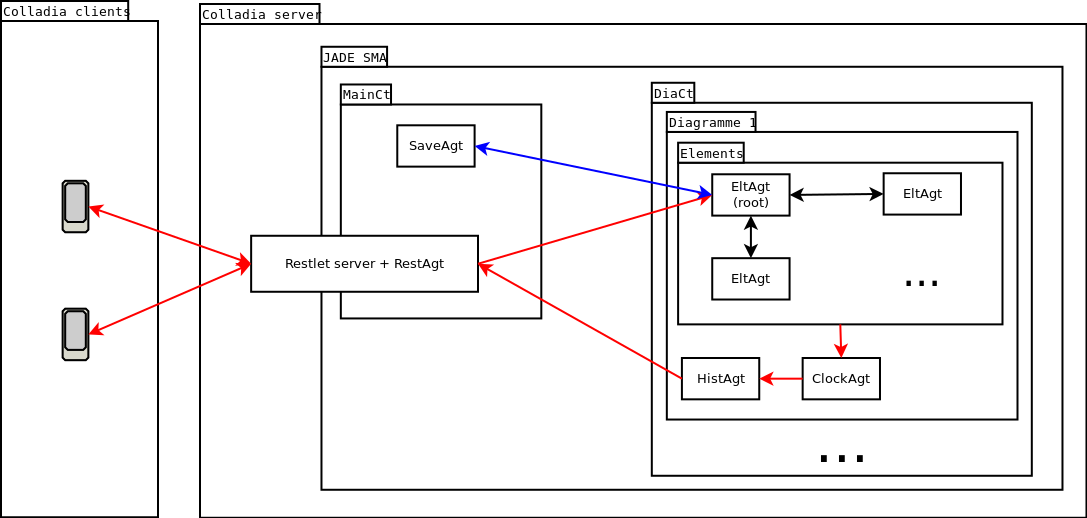
\includegraphics[width=.95\textwidth]{img/general_server}
	\caption{Schéma générale du serveur}
\end{figure}

\subsection{Description de l'interface REST}

\subsection{Description des agents et des comportements}

\subsection{Description générale des messages}

\subsection{Description détaillée des fonctionnalités}
